\documentclass[10pt]{article}
\usepackage{tikz}
\usepackage[margin=0cm]{geometry}
\pagestyle{empty}

\begin{document}

\vspace*{\fill}
\begin{center}
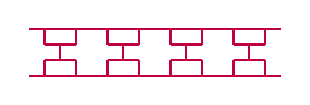
\begin{tikzpicture}[x=0.2cm, y=-0.2cm, thick, purple]
% North to South lines
    \draw (1,0) -- (1,1);
    \draw (1,2) -- (1,3);
    \draw (2,1) -- (2,2);
    \draw (3,0) -- (3,1);
    \draw (3,2) -- (3,3);
    \draw (5,0) -- (5,1);
    \draw (5,2) -- (5,3);
    \draw (6,1) -- (6,2);
    \draw (7,0) -- (7,1);
    \draw (7,2) -- (7,3);
    \draw (9,0) -- (9,1);
    \draw (9,2) -- (9,3);
    \draw (10,1) -- (10,2);
    \draw (11,0) -- (11,1);
    \draw (11,2) -- (11,3);
    \draw (13,0) -- (13,1);
    \draw (13,2) -- (13,3);
    \draw (14,1) -- (14,2);
    \draw (15,0) -- (15,1);
    \draw (15,2) -- (15,3);
% North-West to South-East lines
% West to East lines
    \draw (0,0) -- (16,0);
    \draw (1,1) -- (3,1);
    \draw (5,1) -- (7,1);
    \draw (9,1) -- (11,1);
    \draw (13,1) -- (15,1);
    \draw (1,2) -- (3,2);
    \draw (5,2) -- (7,2);
    \draw (9,2) -- (11,2);
    \draw (13,2) -- (15,2);
    \draw (0,3) -- (16,3);
% South-West to North-East lines
\end{tikzpicture}
\end{center}
\vspace*{\fill}

\end{document}
